\section{Methodology}
\subsection{Data Preprocessing:}
\begin{itemize}
	\item Silence and Noise Removal\\
	Doing a spot check on both training and testing set, we discovered that there exists silence or noise at the beginning of most audio files. We removed those silence or noise parts by calculating the average loudness of each audio file, and recursively comparing the value of 30\% of average loudness to first $\frac{3}{4}$ of the audio file.\\
	\item Equalizing Loudness:\\
	We also figured out that ,between training set and testing sets, there is a loudness difference not representative of class label. So, we linearly equalized average loudness of each file by the average loudness of all audio files. \\
\end{itemize}
\subsection{Feature Extraction:}
\begin{itemize}
	\item Zero Crossing Rate(ZCR):\\
	The rate of sign-changes of the signal during the duration of a particular frame.\cite{b1}We calculate ZCR by equation: $\frac{1}{T-1}\sum_{t = 1}^{T - 1}(s_t s_{t-1})$ where s is single with length T.\\
	\item Energy:\\
	The sum of squares of the signal values, normalized by the respective frame length.\cite{b2} We calculate EE by equation: Energy = $W_{potential} + W_{kinetic} = \int_{V}^{} \frac{p^2}{2p_0c^2} dV + \int_{V}^{} \frac{pv^2}{2}dV$.\\
	\item Entropy of Energy(EE):\\
	The entropy of sub-frames' normalized energies. It can be interpreted as a measure of abrupt changes.\cite{b2} Setting number of short blocks n to 10, we calculate EE by equation: EE = $\frac{(\frac{L}{n})^2}{Eol +eps} \log_{2}({(\frac{(\frac{L}{n})^2}{Eol +eps} + eps})$, where L is the length of audio frame, eps is the learning rate and Eol is the total energy of this frame.\\
	\item Spectral Centroid(SC):\\
	It indicates where the "center of mass" of the spectrum is located. Perceptually, it has a robust connection with the impression of "brightness" of a sound.\cite{b3} We calculate SC through equation: SC = $\frac{\sum_{n = 0}^{N - 1} f(n)x(x)}{\sum_{n = 0}^{N - 1} x(n)}$, where f(n) is the frequency of current bin and x(n) is weighted frequency value.\\
	\item Spectral Energy(SE):\cite{b1}\\
	Entropy of the normalized spectral energies for a set of sub-frames.\cite{b3}. We calculate SE through equation: SE = $\sum_{i = 1}^{N} \frac{1}{N} |X(w_i)|^2$ \\
	\item Spectral Spread(SS):\\
	The second central moment of the spectrum.\cite{b3}. With SC, we can calculate SS by equation: SC = $\sqrt{\frac{\sum_{k = 0}^{\frac{N}{2}} (f_k-SC)^2 |X(k)|^2}{\sum_{k = 0}^{\frac{N}{2}} |X(k)|^2 }}$\\
	\item Spectral Entropy:\\
	Entropy of the normalized spectral energies for a set of sub-frames.\cite{b3} We calculate Spectral Energy by equation : Spectral Entropy = $-\sum_{i = 1}^{n} \frac{\frac{1}{N} |X(w_i)|^2}{\sum_{i}^{}\frac{1}{N} |X(w_i)|^2} \ln\frac{\frac{1}{N} |X(w_i)|^2}{\sum_{i}^{}\frac{1}{N} |X(w_i)|^2}$.\\
	\item Spectral Flux:\\
	The squared difference between the normalized magnitudes of the spectra of the two successive frames.\cite{b3} We calculate Spectral Flux by equation: Spectral Flux = $\int_{\pi_+}^{} I * \cos(\theta(n)) dw(n)$, where I is indicator function of integration that extends only over the solid angles of relevant hemisphere, $\theta(n)$ donates the angle between n and prescribed direction. \\
	\item Spectral Rolloff:\\
	The frequency below which 90\% of the magnitude distribution of the spectrum is concentrated.\cite{b3} We calculate Spectral Rolloff through equation : Spectral Rolloff = arg min$\sum_{i = 1}^{f_c} m_i \geq \sum_{i = 1}^{N}0.9 m_i$, where $f_c$ is the rolloff frequency and $m_i$ is the magnitude of the i-th frequency component of the spectrum. \\
	\item Mel Frequency Cepstral Coefficients(MFCCs):\\
	Mel Frequency Cepstral Coefficients form a cepstral representation where the frequency bands are not linear but distributed according to the mel-scale.\cite{b4} We calculate MFCC by equation: MFCC = $\sum_{k = 0}^{\frac{N}{2}}\log |s(n)| H_i(k\frac{2\pi}{N_p})$, where N is the frame length, s(n) is DFT signal, $H_i$ is the critical band filter at i-th coefficient, and $N_p$ is the number of points used in the short term DFT.\\
	\item Chroma Vector:\\
	A 12-element representation of the spectral energy where the bins represent the 12 equal-tempered pitch classes of western-type music (semitone spacing).\cite{b5} We calculate this by detecting the tone height and chroma of certain segment , and assign each element the vector it falls into.\\
	\item Chroma Deviation:\\
	The standard deviation of the 12 chroma coefficients.\cite{b5}\\
	\item Local Amplitude Minimum:\\
	The number of local minimum amplitude peaks. We extract this feature by counting the number of frames where its frequency derivative is 0.\\
\end{itemize}
First 13 features are widely used in the field of machine learning for audio classification. We utilize an existing library\cite{b6} that implements first those features. The last feature Local Amplitude Minimum is introduced by us to help classifiers distinguishing normal audio and abnormal audio, which turns out to be extremely efficient. \\
\subsection{Validation Method:}
Before mentioning detailed structure and algorithm we have attempted, I want to point out that we measure accuracy using stratified 10-fold cross validation(CV). Any classifier's accuracy is the weighted average accuracy of numbers we get from 10 folds.  \\
\indent However, for transductive learning algorithm such as Transductive Support Vector Machine or Label Propagation, we could not do cross validation since there is no validation set for transductive learning. Accuracy we have on those algorithms is the accuracy on whole training set, in other word, the rate of convergence. 
\subsection{Attempted Algorithms:}
Tree-Based Algorithms:
\begin{itemize}
	\item Decision Tree:\\
	Utilizing tree structures, decision tree algorithm calculates entropy of each feature and splits node based on the rank of features with respect to their entropies. Probably due to the fact that different classes are representative in different features and skewed class distribution, a single decision tree could not solve this learning problem and we only get 62\% accuracy on CV.\\
	\item Random Forest:\\
	Instead of having a single tree structure, Random Forest fits a number of decision tree classifiers on various sub-samples of the dataset.\cite{b7} Using Random Forest classifier, we get 89\% accuracy on CV. But even with such high accuracy, Random Forest performs poorly on test set according to the feedback from oracle. We analyze that the differences on performance between training set and testing set probably result from skewed data distribution and over-fitting. \\
\end{itemize}

\indent Based on cross validation results on experiments we have done, it seems like tree-based algorithm generally is inappropriate for this learning task. \\

Support Vector Machines(SVMs):\\
\begin{itemize}
	\item Linear SVM:\\
	Based on the features' distribution of each training example, SVM differentiates classes by building a hyperplane that maximizes the margin between classes. And for Linear SVM, the decision boundary is a linear function. After tuning loss penalty and class weight, we get 91\% accuracy on CV and a relatively reasonable classification on test set according to the feedback from oracle.\\
	\item SVM with Radial Basis Function kernel(SVM-RBF):\\
	Pretty similar to Linear SVM, SVM-RBF differs by the non-linear kernel function. After having a reasonable result from Linear SVM, we were excited on trying SVM-RBF(with tuned loss penalty and gamma). It ends up having 89\% on CV and similar test set performance. However in the late phase, we discarded SVM-RBF because with the number of features we have, it is possible that a non-linear kernel function over-fits. \\
\end{itemize}

Transductive Learning Algorithms:\newline\\
\indent Noticing that size of test set is twice size of training set, in order to get better generalization, we want to utilize test set and attempted several transductive learning algorithms. \\
\begin{itemize}
	\item Label Propagation:\\
	Identifying the test example's closest training set neighbor, Label Propagation assigns the same label that neighbor has to the test example. Without CV on this algorithm, we compare the number of assigned labels of each class to that from SVMs. From Label Propagation, we get 69 Normals, 107 Vocal Palsys and 171 Phonotraumas. From Linear SVM, we get 65 Normals, 79 Vocal Palsys and 167 Phonotraumas.\\
	\item Transductive Support Vector Machine(TSVM):\\
	This is a SVM-RBF based classifier with test set regulating the range of how far away the hyperplane can extends. Although in test set, TSVM overcalls a great number of Normal, it could give us a board view of all 'Normal-ish' examples, and later on we could limit our focus on this specific set of Normals. \\
\end{itemize}

Multiple Instance Learning Regression(MILR):\\
\begin{itemize}
	\item 
	Instead of receiving a set of instances which are individually labeled, the learner receives a set of labeled bags, each containing many instances. In the simple case of multiple-instance binary classification, a bag may be labeled negative if all the instances in it are negative. On the other hand, a bag is labeled positive if there is at least one instance in it which is positive. \cite{b10} Although MILR undercalls Normal, having super high Area under ROC Curve(AUC) 0.92, MILR could work as an oracle and we only focus on test examples labeled with confidence higher than 85\%.\\
\end{itemize}
\subsection{Final Architecture Overview:}
	Our whole model-building infrastructure is based on scikit-learn\cite{b7}\cite{b8}. \\
	\indent We tried Support Vector Machine, Boosting, Random Forest, Extratrees, Multiple Instance Learning, Label Propagation. After few experiments, it seemed like tree algorithms performed poorly on this task and we finalized our focus on SVM, Label Propagation, SVM-RBF and MILR with pipeline. Any single classifier undercalled Normal and Neoplasm patients, which we think is resulted from different class distributions between training and testing set. \\
\indent So, we converted this relatively complex learning task into three less complicated tasks: Normal vs. Pathological, Vocal vs. Rest of Diseases, and Phonotrauma vs. Neoplasm, with each learning task having ensemble consisted of 4 classifiers.[Fig. 1] The reason why we design the pipeline this way is based on the difficulty of classification according to our perception. (From easiest Normal vs. Pathological to hardest Phonotrauma vs. Neoplasm)\\
	\begin{figure}[!htbp]
		\begin{center}
			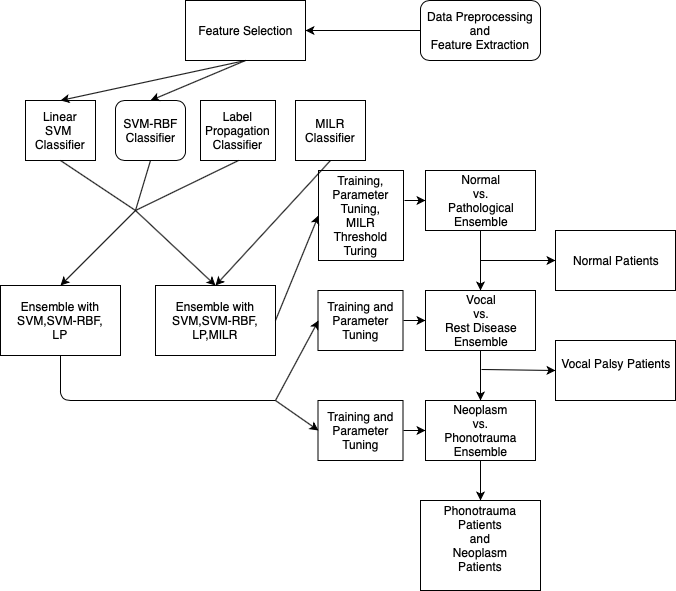
\includegraphics[scale=0.35]{Diagram_3.png}
		\end{center}
		\caption{Pipeline Ensemble}
	\end{figure}

\subsection{Feature Selection:}
Due to the fact that the size of our training set is relatively small, in case of over-fitting, for each classifier we select 50\% best features, with respect to entropy. However, it seems like feature selection jeopardizes the performance of transductive learning. So we only utilize feature selection on SVM and SVM-RBF.

\subsection{Hyper Parameter Tuning:}
Since the size of training set is getting smaller and smaller as we propagate through the pipeline, in order to get trustworthy accuracy to tune parameter for SVC, for all three ensembles, we use the same parameter tuned in the first ensemble. The process is pretty straightforward; we simply set up two loops, one of which for C and one of which for gamma. The tuned parameters are 10 for C, and 0.01 for gamma. Also due to the skewed distribution in training set, we modify the class weight with respect to the proportion of class. 


